\begin{figure}[!ht]
    \centering
    \begin{subfigure}[t]{0.3\textwidth}
        \centering
        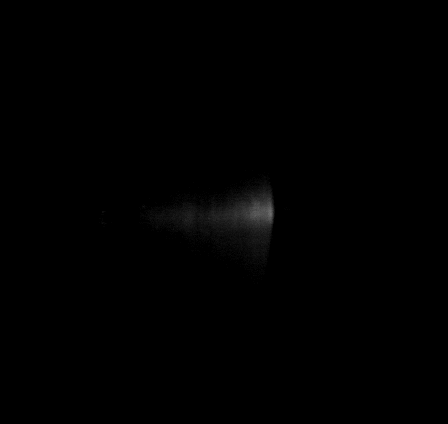
\includegraphics[width=\textwidth]{assets/4 experiments/CW LSP frames Photron/LSP385_V2_CW1_Fr48.png}
        \caption{\qty{4.8}{ms}}
        %\label{fig:V1_ignition_frames_16}
    \end{subfigure}
    \hfill
    \begin{subfigure}[t]{0.3\textwidth}
        \centering
        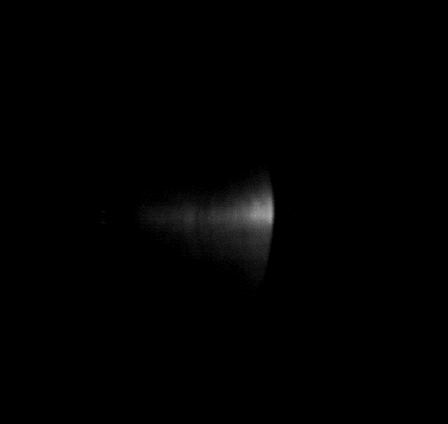
\includegraphics[width=\textwidth]{assets/4 experiments/CW LSP frames Photron/LSP385_V2_CW1_Fr250.png}
        \caption{\qty{25.0}{ms}}
        %\label{fig:ignition_frames_17}
    \end{subfigure}
    \hfill
    \begin{subfigure}[t]{0.3\textwidth}
        \centering
        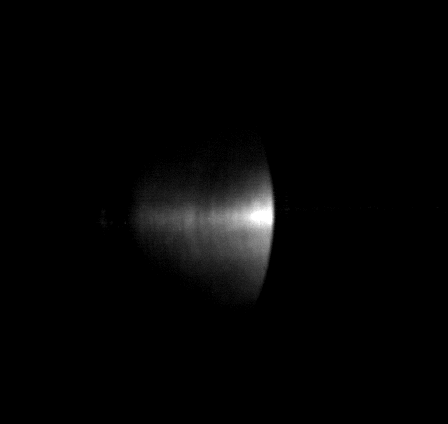
\includegraphics[width=\textwidth]{assets/4 experiments/CW LSP frames Photron/LSP385_V2_CW1_Fr508.png}
        \caption{\qty{50.8}{ms}}
        %\label{fig:ignition_frames_18}
    \end{subfigure}
    \caption{First CW LSP captured by the Photron high-speed camera: \qty{342}{W}, \qty{20.0}{bar}. LSP385\_V2\_CW1.}
    \label{fig:CW_V2_Photron_frames}
\end{figure}

% The brightness of the plasma reaches its maximum intensity around 50 ms, and this brightness is constant for 10 ms. A flickering of the LSP is seen between at 70.0 ms, before it dies down and is completely extinguished after 88.3 ms.